%----------------------------------------------------------------------------------------
%	PACKAGES AND OTHER DOCUMENT CONFIGURATIONS
%----------------------------------------------------------------------------------------

\documentclass[a4paper]{scrartcl}
\usepackage[english]{babel}
\usepackage[utf8]{inputenc}
\usepackage{amsmath}
\usepackage{graphicx}
\usepackage{caption}
\usepackage{subcaption}
\usepackage[colorinlistoftodos]{todonotes}
\addtokomafont{disposition}{\rmfamily}

\usepackage{footnote}
\makesavenoteenv{figure}

\usepackage[babel,english=british]{csquotes} % cool quotes
\usepackage[backend=biber]{biblatex} % bibliogrpahy
\addbibresource{literature.bib}

\begin{document}

\title{fMRI: BOLD-Contrast and neural activity imaging}
\subtitle{Master Pflichtseminar}
\author{Lucas-Raphael Müller}
% \date{\today}
\maketitle

\begin{abstract}
Your abstract.
\end{abstract}

\tableofcontents

\newpage

\section{Introduction}
\label{sec:intro}

\subsection{Outline}
\subsection{What's the aim?}

\section{Physiology}
Not only is the knowledge of the functional structure of the human brain a major issue for neuroscientists, it's vast complexity is also fascinating for almost everyone.
Major parts of the brain consists of neurons. 
Biophysical aspects are understood on a neuron-wise context, membrane potentials, ion channels and signal propagation are topics to be found in all physiology books which are worth the paper they have been printed on.\cite[577 et. seq.]{guyton}
% Commands to include a figure:

\begin{figure}[ht]
\begin{subfigure}[l]{0.35\textwidth}

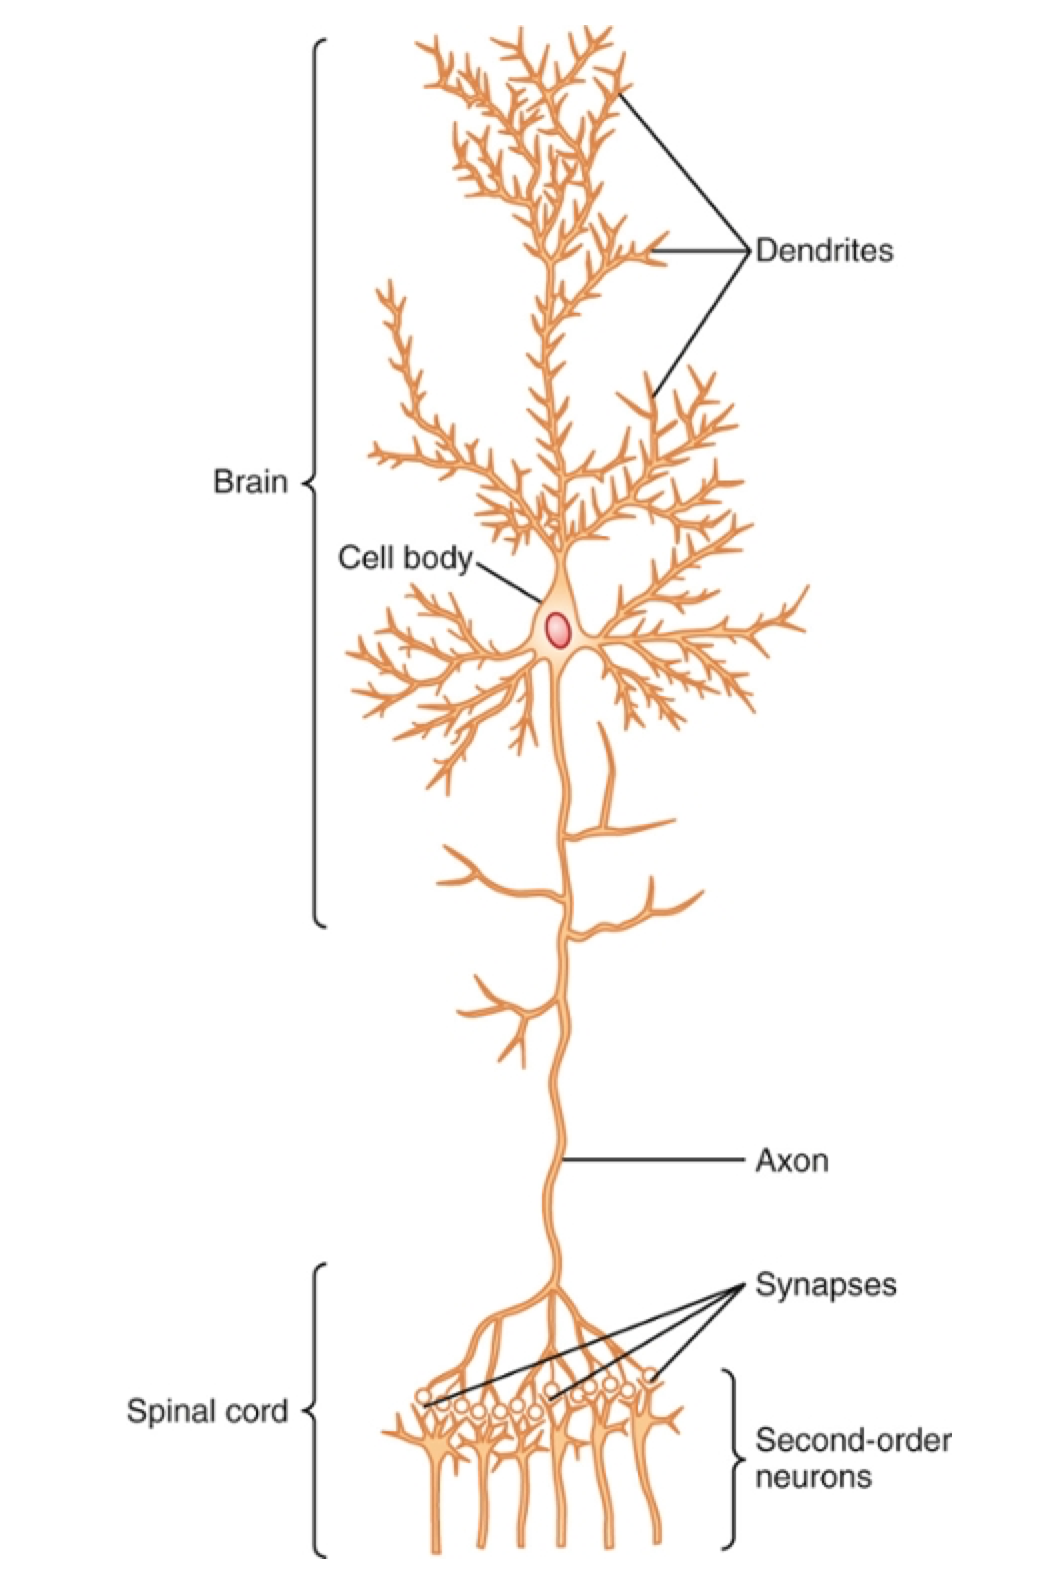
\includegraphics[width = \textwidth]{pictures/largeNeuron.png}
\subcaption{Structure of a large neuron in the brain showing it's important functional parts.\cite[578]{guyton}}

\end{subfigure}
\begin{subfigure}[r]{0.6\textwidth}
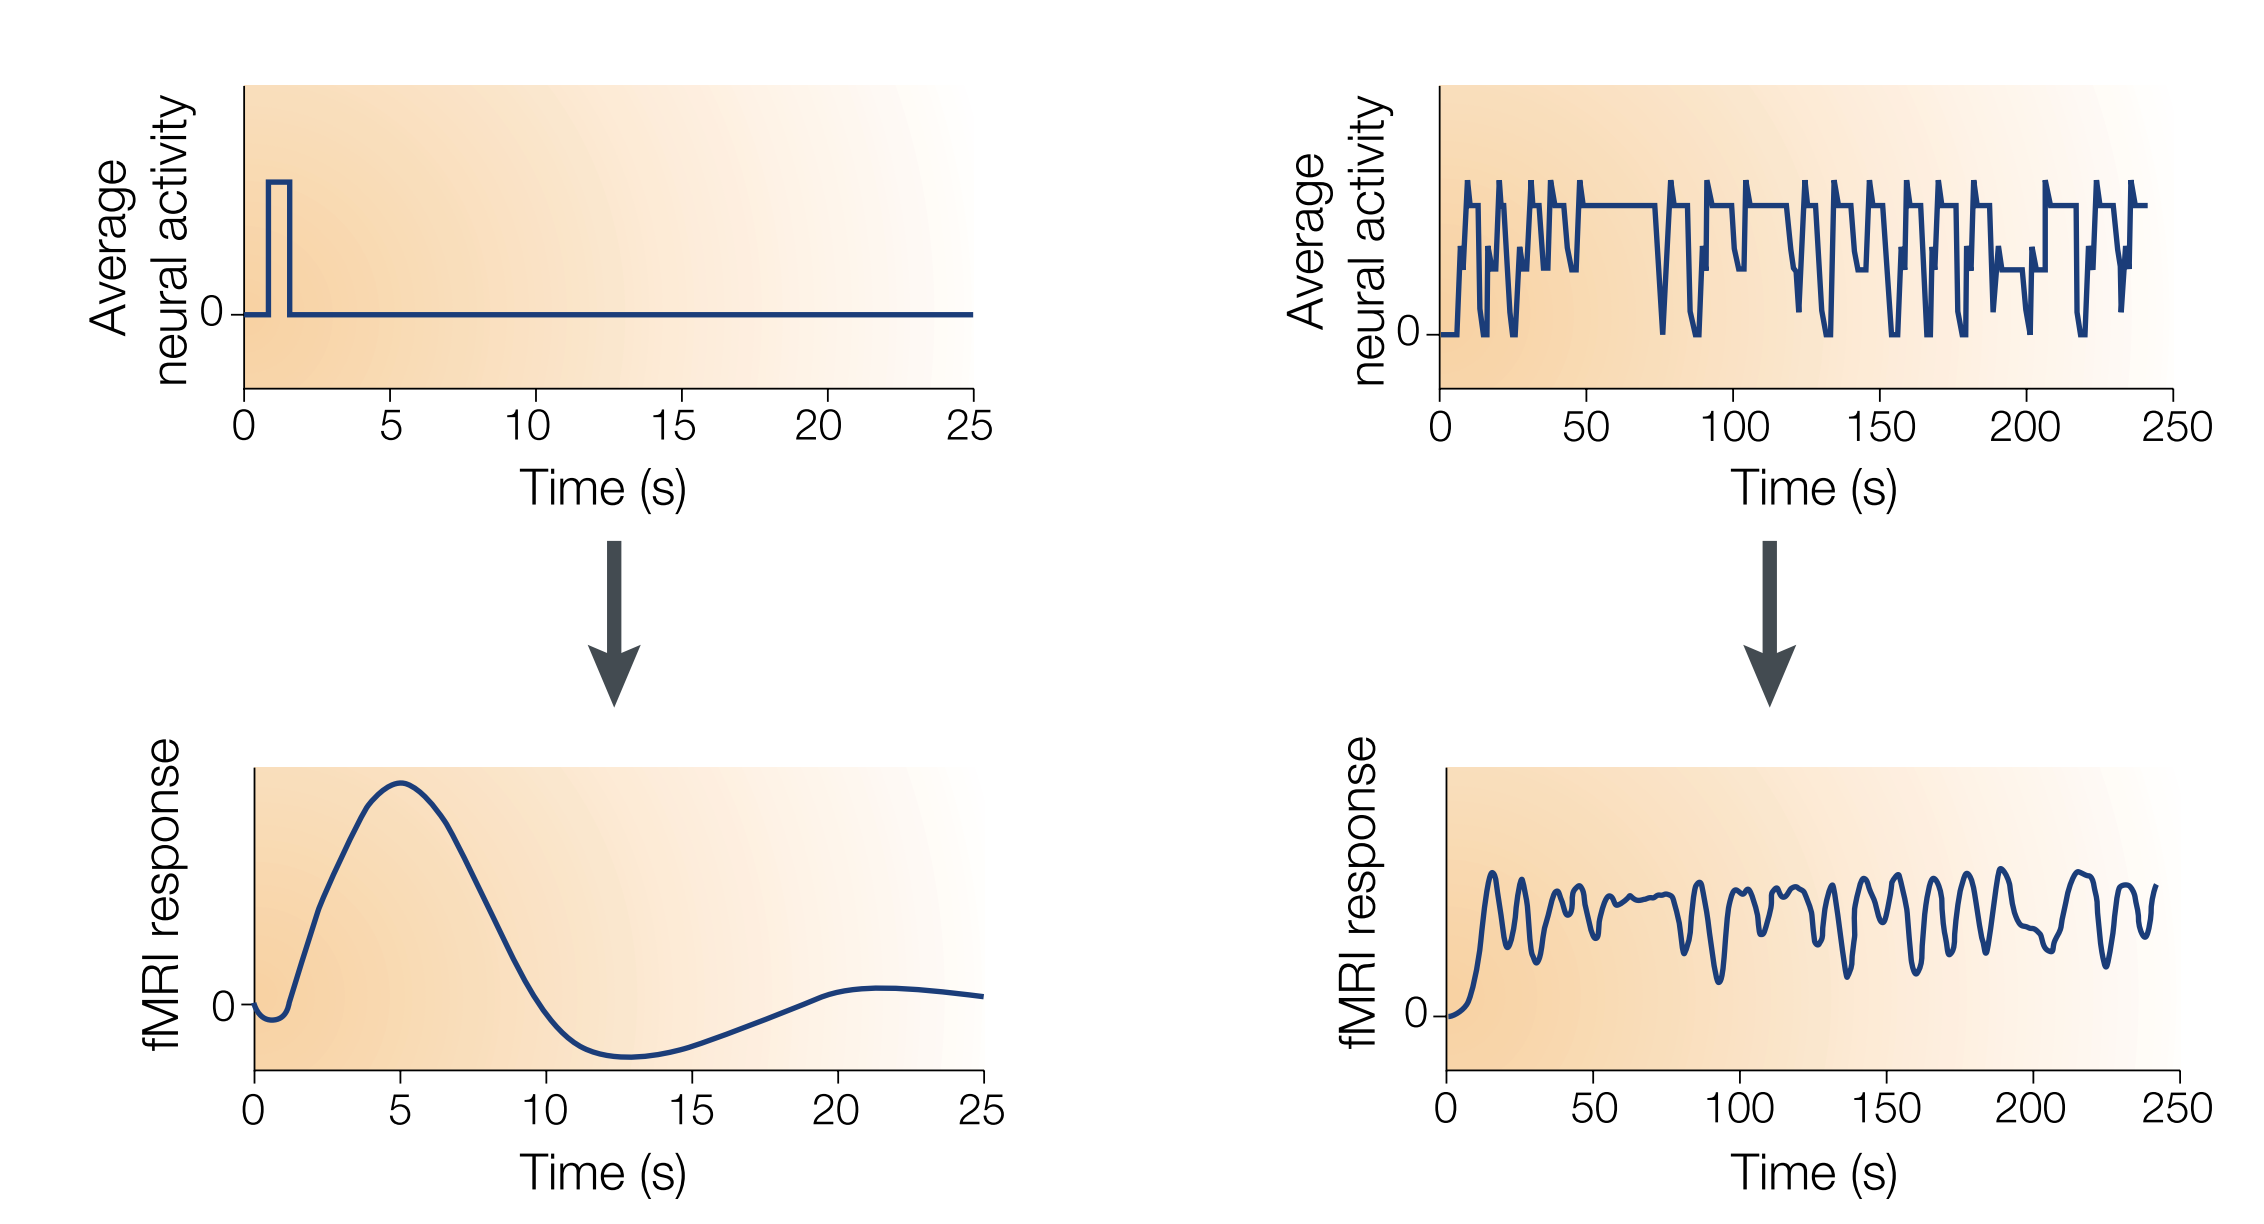
\includegraphics[width = \textwidth]{pictures/signalProcessing.png}
\subcaption{Top row: hypothetical plots of average neuronal activity over time. Bottom row: corresponding functional magnetic resonance imaging (fMRI) responses. Left: hypothetical haemodynamic impulse response function (HIRF) measured as the response to a brief pulse of neuronal activity. Right: the fMRI response when the average neuronal activity alternates (at specific times) between three different states.\cite{Heeger2002}}
\end{subfigure}
\caption{Zwei Bilder mit Subfigure nebeneinander}
\end{figure}

Being aware that a physical description is possible on a microscopic scale, it is a task of huge complexity to describe neural activity in total.
Direct measurement of neural activity, i.e. placing eletrodes directly in the brain, requires surgery and most of the time this can only be done in animal experiments. 
Information can be received at the scalp of the brain, however this is a rather rough estimation and not useful for drawing precise activation maps.\cite[6]{buxton}
Modern approaches are positron emission tomography (PET) or funtional magnetic resonance imaging among others.
These methods rely on a implicit measurement, as no electrical field or voltage drop is measured, but other quantities which are followup-like, namely glucose consumption or blood oxygenation level, which are again measured implicitly.
In the former case, tracers with glucose accumulate in regions of high glucose consumption resulting in a local higher active radiation source.
In the latter case, blood oxygenation level changes local inhomogenities of the magnetic field and leads to different \textit{T2*} relaxation.
The author wants to focus on aspects of the latter one and shortly describe important underlying principles as well as the most basic but necessary physiological knowledge.
With ongoing progress in medical physics research promising measurement method \textit{Magnetoencephalography (MEG)} with great spatial and temporal resolution is mentioned briefly in \ref{sec:outlook}. 

\subsection{Neural Activity}


Notes:
Deoxy is paramagnetic, induces magnetic field inhomogenity \\
Oxy is diamagnetic, no influence \\
Cerebal blood flow. Brain activity -. blood flow -. oxygenated hemoglobin -. $T_2^*$ -. MRI signal

\section{Hardware}
\label{sec:hardware}

\section{Sequence and Signal}
\label{sec:sequenceSignal}

\section{Software}
\label{sec:software}

\section{Real example (me)}
\label{sec:example}

\section{Outlook}
\label{sec:outlook}

\printbibliography

\end{document}

\begin{table}
\centering
\begin{tabular}{l|r}
Item & Quantity \\\hline
Widgets & 42 \\
Gadgets & 13
\end{tabular}
\caption{\label{tab:widgets}An example table.}
\end{table}
